 \documentclass[a4paper,11pt]{article}

\usepackage{amsmath}
\usepackage{amssymb}
\usepackage{amsthm}
\usepackage{graphicx}
\usepackage{caption}
\usepackage{subcaption}

\newtheorem{thm}{Theorem}
\newtheorem{lem}{Lemma}

\newcommand{\beq}{\begin{equation}}
\newcommand{\eeq}{\end{equation}}

\newcommand{\ba}{\begin{array}}
\newcommand{\ea}{\end{array}}

\newcommand{\bea}{\begin{eqnarray}}
\newcommand{\eea}{\end{eqnarray}}

\newcommand{\bc}{\begin{center}}
\newcommand{\ec}{\end{center}}

\newcommand{\ds}{\displaystyle}

\newcommand{\bt}{\begin{tabular}}
\newcommand{\et}{\end{tabular}}

\newcommand{\bi}{\begin{itemize}}
\newcommand{\ei}{\end{itemize}}

\newcommand{\bd}{\begin{description}}
\newcommand{\ed}{\end{description}}

\newcommand{\bp}{\begin{pmatrix}}
\newcommand{\ep}{\end{pmatrix}}

\newcommand{\p}{\partial}
\newcommand{\sech}{\mbox{sech}}

\newcommand{\cf}{{\it cf.}~}

\newcommand{\ltwo}{L_{2}(\mathbb{R}^{2})}
\newcommand{\smooth}{C^{\infty}_{0}(\mathbb{R}^{2})}

\newcommand{\br}{{\bf r}}
\newcommand{\bk}{{\bf k}}
\newcommand{\bv}{{\bf v}}

\newcommand{\gnorm}[1]{\left|\left| #1\right|\right|}
\newcommand{\ipro}[2]{\left<#1,#2 \right>}
\title{Long Shallow Waves in Density Stratified, Bilinear Shear Currents.}
\author{C.W. Curtis, K. Oliveras, T. Morrison, S. Reeves}
\date{}
\begin{document}
\maketitle
\section{Introduction}
Given the role ocean currents play in moving materials and energy throughout the ocean, they are the subject of much study and interest \cite{young1}.  This paper focuses on shear currents, which can be thought of as arising from air/wind interactions \cite{miles,valenzuela,young2} that can give rise to shear currents beneath the surface of the fluid \cite{banner,dasilva}.  Shear currents also arise from viscosous effects along sea beds \cite{dasilva}. Likewise, the impact of temperature and salinity variation leads to the formation of rapid transitions in density throughout the ocean which support the formation of large internal waves, while in atmospheric contexts inversion layers can support internal wave propagation.  It is a natural question then to examine the role currents play in density stratified flows and how shear currents influence the propagation of surface and internal waves.  

In the abscence of density stratifitcation, the impact of shear currents on surface waves and bulk-flow is a well-studied problem.  Starting with the seminal paper of Benjamin \cite{benjamin}, which looked at small-amplitude nonlinear steady waves over arbitrary vertical shear flows, research has shown that on linearly varying shear currents can induce solitary and even overturning waves \cite{dasilva,choi,freeman,simmen,vandenbroeck}, inviscid eddy-formation \cite{dasilva,miroshnikov}, and non-monotone pressure distributions \cite{dasilva,ali,oliveras}.  A large body of rigorous results concerning the existence and properties of steady periodic waves over linearly varying shear currents has appeared as well.  See \cite{constantin} and its extensive bibliography for reference.  Beyond linearly varying shear currents, again we note \cite{benjamin} was clearly ahead of its time, while \cite{ko} numerically examines the impact of shear currents with non-constant vorticity on steady waves.  Nonsteady wave propagation has been looked at first in \cite{dalrymple}, experimentally and numerically in \cite{swan}, and recently in \cite{nwogu}, which looks at fully three-dimensional profiles.  We make particular note of \cite{dalrymple}, which was the first paper to examine the case of a bilinear shear flow, in which the vorticity has a discontinuous jump between two constant values at different depths of the fluid.  

Throughout all of the listed works, a key feature is the presence or lack thereof of stagnation points in the flow.  These are points at which travelling wave speeds exactly match the background shear velocity, and a type of resonance occurs when stagnation points are present.  Stagnation points are responsible for the eddy formation and layer separation seen in \cite{dasilva}, while \cite{benjamin} notes that stagnation points should prevent the formation of steady solitary wave profiles.  As shown in \cite{oliveras}, the presence of stagnation points, and their clear identification, is critical in understanding bulk flow properties and maintaing physical constraints of the fluid models.  

Density stratified shear flows have likewise received much attention over the years.  In parallel with the description of bilinear shear currents, we refer to fluid systems composed of two fluids of differing, but constant densities, as bistratified fluids.  Nonlinear, large amplitude steady waves for bistratified fluids were studied in \cite{pullin2,pullin4}, the KdV and Benjamin--Ono equations were derived as models of long waves in the presence of arbitrary shear and density variations \cite{maslowe}.  In \cite{milewski}, unsteady, large amplitude nonlinear waves are examined in bistratified fluids.  As shown throughout these papers, strong internal waves are found, and a complete characterization of the linear stability of small amplitude internal waves in the presence of a bilinear shear current \cite{pullin3}.   As noted in \cite{maslowe}, given the interest in and importance of internal solitary waves in oceanic flows \cite{appel,zhao}, an understanding of the influence of shear currents is necessary to better model flow through channels, estuaries, or relatively shallow water environments \cite{farmer}.  

However, previous works on stratified shear flow have usually focused on internal layers alone by either assuming rigid lids both above and below the fluid \cite{pullin2,pullin4,milewski,pullin3}, or by taking boundaries to infinity \cite{maslowe}.  Therefore, in this paper we look at the evolution of a free surface and a free internal layer for a bilinear shear current in a bistratified fluid.  See Figure \ref{fig:surface} for reference.  
\begin{figure}[t]
\centering
\includegraphics[width=.4\textwidth]{surface_wave}
\caption{A bilinear shear current, characterized by constant vorticities $\omega_{j}$, in a bistratified fluid, characterized by fluid densities $\rho_{j}$.  The resting fluid depths are $z=H$, $z=0$, and the bottom boundary is at a depth $z=-h$.}
\label{fig:surface}
\end{figure}
Using the techniques in \cite{ashton,haut}, a closed system describing the evolution of the two free surfaces and their corresponding velocity potentials are derived.  

Using a shallow water, long wavelength ansatz, the flow is separated into four separate waves characterized by four different wave speeds and four uncoupled Korteweg--de Vries (KdV) equations describing the long time evolution of each separated wave.  While exact formulas for the wave speeds and KdV coefficients are not given due to their complexity, they are readily computed numerically, and characterizations of each value as functions of the stratification $\rho = \rho_{2}/\rho_{1}$ and the vorticities $\omega_{j}$ are given.  As we show, the full range of phenomena one finds in the KdV equation, i.e. soliton trains, undular bores, and dispersive scattering, manifests itself in the surface and internal layer flows.  Our results show that generically solitons only form for depression waves, whereas elevated packets generally separate out into dispersive trains or undular bores.

\subsection{Problem Formulation}

We now examine the case of unsteady nonlinear wave propagation over a bilienar, density stratified, shear current.  We otherwise assume the fluid to be incompressilbe and invisicid with the only external force being that of gravity.  We suppose that the top fluid has a free surface, say $z=\eta_{1}(x,t)+H$, and the interface, say $z=\eta_{2}(x,t)$, between the two fluids is also free.  We suppose that there is a flat bottom at $z=-h$ through which no fluid flows.  See Figure \ref{fig:surface} for reference. 

We have the fluid velocities in each region, say ${\bf u}_{j}$, given by 
\[
{\bf u}_{j} = \omega_{j}z\hat{{\bf x}} + \nabla \varphi_{j}, 
\]
where we take $\varphi_{j}$ to be a harmonic function in each layer.  We likewise define the corresponding stream functions $\psi_{j}$ such that 
\[
\p_{x}\psi_{j} = \p_{z}\varphi_{j}, ~ -\p_{z}\psi_{j} = \omega_{j}z + \p_{x}\varphi_{j}.
\]
This is equivalent to defining 
\[
{\bf u}_{j} = (-\p_{z}\psi_{j},0,\p_{x}\psi_{j})^{T}, 
\]
which ensures that $\nabla \cdot {\bf u}_{j} = 0$, or incompressibility is maintained, in each region of constant density.  

If we take the density and vorticity in each region to be given by $\rho_{j}$ and $\omega_{j}$, then we have the following Bernoulli equations describing the flow:
\[
\p_{t}\varphi_{j} + \frac{1}{2} \left( (\p_{x}\varphi_{j}+\omega_{j}z)^{2} + (\p_{z}\varphi_{j})^{2} \right) + \omega_{j}\psi_{j} +  \frac{1}{\rho_{j}} p_{j} + gz =C(t).
\]
At each free surface one has, allowing for a slight abuse of notation, 
\[
\p_{x} \psi_{j}(x,\eta_{j}(x,t),t) = \p_{x}\psi_{j} + \p_{z}\psi_{j}\p_{x}\eta_{j}.
\]
As long as the surfaces remain single valued, we have that 
\[
\frac{dz}{dt} = \p_{x}\psi_{j} = \p_{x}\eta_{j}\p_{z}\psi_{j} + \p_{t}\eta_{j}.
\]
Therefore, we can formally define 
\[
\psi_{j}(x,\eta_{j}(x,t),t) = \p_{x}^{-1}\p_{t}\eta_{j}.
\]

Matching each layer via the pressure, and taking the pressure at the topmost surface to be constant, we then get the bulk incompressibility conditions 
\[
\ba{lr}
\Delta \varphi_{1} = 0, & \eta_{2}(x,t) < z < \eta_{1}(x,t) +H\\ 
\Delta\varphi_{2} = 0, & -h<z<\eta_{2}(x,t)\\
\ea
\]
the kinematic boundary conditions
\[
\ba{rl}
\p_{t}\eta_{1} - \p_{z}\varphi_{1} + (\p_{x}\varphi_{1}+\omega_{1}(\eta_{1}+H))\p_{x}\eta_{1}=0,  & z = \eta_{1}(x,t)+H\\
\p_{z}\varphi_{2} = 0,  &z=-h\\
\p_{t}\eta_{2} - \p_{z}\varphi_{2} + (\p_{x}\varphi_{2}+\omega_{2}\eta_{2})\p_{x}\eta_{2}=0,  & z = \eta_{2}(x,t),
\ea
\]
and the two Bernoulli equations 
\[
\p_{t}\varphi_{1} + \frac{1}{2} \left( (\p_{x}\varphi_{1}+\omega_{1}(\eta_{1}+H))^{2}-\omega^{2}_{1}H^{2} + (\p_{z}\varphi_{1})^{2} \right) + \omega_{1}\p_{x}^{-1}\p_{t} \eta_{1} + g\eta_{1} = 0,
\]
and
\begin{align*}
\rho_{1}\left(\p_{t}\varphi_{1} + \frac{1}{2} \left( (\p_{x}\varphi_{1}+\omega_{1}\eta_{2})^{2} + (\p_{z}\varphi_{1})^{2} \right) + \omega_{1}\p_{x}^{-1}\p_{t} \eta_{2} + g\eta_{2} \right) = \\
\rho_{2}\left(\p_{t}\varphi_{2} + \frac{1}{2} \left( (\p_{x}\varphi_{2}+\omega_{2}\eta_{2})^{2} + (\p_{z}\varphi_{2})^{2} \right) + \omega_{2}\p_{x}^{-1}\p_{t} \eta_{2} + g\eta_{2} \right) + \sigma\frac{\p_{x}^{2}\eta_{2} }{(1+(\p_{x}\eta_{2})^{2})^{3/2}}.
\end{align*}
at $z=\eta_{1}(x,t)+H$ and $z=\eta_{2}(x,t)$ respectively.  We point out that it would be natural to include surface tension in both Bernoulli equations, though we omit this for the time being.  

We define the surface potentials 
\[
Q(x,t) = \varphi_{1}(x,\eta_{1}(x,t)+H,t), ~ q_{1}(x,t) = \varphi_{1}(x,\eta_{2}(x,t),t), ~ q_{2}(x,t) = \varphi_{2}(x,\eta_{2}(x,t),t), 
\]
and note that we have transformation
\[
\left.\nabla \varphi_{1}\right|_{z=\eta_{1}} = \frac{1}{1+(\p_{x}\eta_{1})^{2}}\bp 1 & -\p_{x}\eta_{1} \\ \p_{x}\eta_{1} & 1 \ep\bp \p_{x}Q \\ \p_{t}\eta_{1} + \omega_{1}(\eta_{1}+H)\p_{x}\eta_{1}\ep,
\]
and, at $z=\eta_{2}(x,t)$,
\[
\left.\nabla \varphi_{j}\right|_{z=\eta_{2}} = \frac{1}{1+(\p_{x}\eta_{2})^{2}}\bp 1 & -\p_{x}\eta_{2} \\ \p_{x}\eta_{2} & 1 \ep\bp \p_{x}q_{j} \\ \p_{t}\eta_{2} + \omega_{j}\eta_{2}\p_{x}\eta_{2}\ep.
\]
Likewise, we have 
\begin{align*}
\left.\p_{t}\varphi_{1}\right|_{z=\eta_{1}} = & \p_{t}Q - \p_{t}\eta_{1}\left.\p_{z}\varphi_{1}\right|_{z=\eta_{1}},\\
\left.\p_{t}\varphi_{j}\right|_{z=\eta_{2}} = & \p_{t}q_{j} - \p_{t}\eta_{2}\left.\p_{z}\varphi_{j}\right|_{z=\eta_{2}}, 
\end{align*}
so any bulk potential variable evaluated at the surface can be transformed to a surface variable.  

\section{The Nonlocal Formulation}

We now introduce the auxillary harmonic functions $\phi$ which gives us the identity, following \cite{afm}, 
\[
\p_{x}\left(\p_{z}\varphi_{j}\p_{x}\phi + \p_{x}\varphi_{j}\p_{z}\phi \right) + \p_{z}\left(\p_{z}\varphi_{j}\p_{z}\phi - \p_{x}\varphi_{j}\p_{x}\phi \right) = 0,
\]
so that using Green's theorem, we have that 
\[
\int_{\p D_{j}} \left(\left(\p_{z}\varphi_{j}\p_{x}\phi + \p_{x}\varphi_{j}\p_{z}\phi \right)n_{1,j} + \left(\p_{z}\varphi_{j}\p_{z}\phi - \p_{x}\varphi_{j}\p_{x}\phi \right)n_{2,j}\right) ds = 0,
\]
where $\p D_{1}$ consists of the curves $z=\eta_{1}$, $z=\eta_{2}$, and the vertical lines $x=\pm L$, $\p D_{2}$ consists of the curves $z=\eta_{2}$, $z=-h$, and the vertical lines $x=\pm L$, $\hat{{\bf n}}_{j}=(n_{1,j},n_{2,j})$ is the unit normal along the path, and $s$ is arc length along the path.  

In $D_{2}$, if we suppose that as $L\rightarrow \infty$ we go to a quiescent fluid, by choosing $\phi = e^{ikx \pm kz}$, we then have two integral equations given by 
\[
\int_{\mathbb{R}}dx ~ e^{ikx+k\eta_{2}}\left(k(\p_{t}\eta_{2} + \omega_{2}\eta_{2}\p_{x}\eta_{2})-ik\p_{x} q_{2}\right) + \int_{\mathbb{R}}dx~e^{ikx-kh}(ik\p_{x}q_{2}) = 0,
\]
and
\[
\int_{\mathbb{R}}dx ~ e^{ikx-k\eta_{2}}\left(-k(\p_{t}\eta_{2} + \omega_{2}\eta_{2}\p_{x}\eta_{2})-ik\p_{x} q_{2}\right) + \int_{\mathbb{R}}dx~e^{ikx+kh}(ik\p_{x}q_{2}) = 0.
\]
Mutiplying the first by $e^{kh}$, the second by $e^{-kh}$, and taking the difference produces the integral equation  
\[
\int_{\mathbb{R}}dx ~ e^{ikx}\left(i\cosh(k(\eta_{2}+h))(\p_{t}\eta_{2} + \omega_{2}\eta_{2}\p_{x}\eta_{2}) + \sinh(k(\eta_{2}+h))\p_{x} q_{2} \right) = 0.
\]

Likewise, in $D_{1}$, if we use the difference of the integral equations obtained by using $\phi = e^{ikx \pm k(z-H)}$, then we get the equation
\begin{align*}
\int_{\mathbb{R}}dx ~ e^{ikx}\left(i\cosh(k\eta_{1})(\p_{t}\eta_{1} + \omega_{1}(\eta_{1}+H)\p_{x}\eta_{1}) + \sinh(k\eta_{1})\p_{x} Q \right) - \\
\int_{\mathbb{R}}dx ~ e^{ikx}\left(i\cosh(k(\eta_{2}-H))(\p_{t}\eta_{2} + \omega_{1}\eta_{2}\p_{x}\eta_{2}) + \sinh(k(\eta_{2}-H))\p_{x} q_{1} \right) = 0.
\end{align*}
Using the difference of the two equations obtained in $D_{1}$ by taking $\phi = e^{ikx \pm kz}$ gives
\begin{align*}
\int_{\mathbb{R}}dx ~ e^{ikx}\left(i\cosh(k(\eta_{1}+H))(\p_{t}\eta_{1} + \omega_{1}(\eta_{1}+H)\p_{x}\eta_{1}) + \sinh(k(\eta_{1}+H))\p_{x}Q \right) - \\
\int_{\mathbb{R}}dx ~ e^{ikx}\left(i\cosh(k\eta_{2})(\p_{t}\eta_{2} + \omega_{1}\eta_{2}\p_{x}\eta_{2}) + \sinh(k\eta_{2})\p_{x} q_{1} \right) = 0.
\end{align*}

We can likewise transform the two Bernoulli equations into their surface variable form, though we avoid explicitly writing these expressions down due to their complexity.  Nevertheless, we now have five surface equations for the five surface variables $\eta_{1}$, $\eta_{2}$, $Q$, $q_{1}$, and $q_{2}$.
%%%%%%%%%%%%%%%%%%%%%%%%%%%%%%%%%%%%%%%%%%%%%%%%%%%%%%%%%%%%%%%%%%%%%%%%%%%%%%%%%%%
\subsection{The Shallow Water Limit: Balanced Depth Case}
%%%%%%%%%%%%%%%%%%%%%%%%%%%%%%%%%%%%%%%%%%%%%%%%%%%%%%%%%%%%%%%%%%%%%%%%%%%%%%%%%%%
We now pass to a shallow-water limit.  By this, we mean that we introduce the non-dimensional variables 
\[
\tilde{x} = x/L,~\tilde{z}=z/H,~ \tilde{t} = \frac{\sqrt{gH}}{L}t,~\tilde{k}=Lk,~ \eta_{j} = a\tilde{\eta}_{j},~ Q = \frac{agL}{\sqrt{gH}}\tilde{Q}, ~ q_{j} = \frac{agL}{\sqrt{gH}}\tilde{q}_{j}, 
\]
and we take the balances
\[
\frac{H}{h} = 1, ~ \frac{a}{H} = \epsilon,  ~ \frac{H}{L} = \gamma, ~ \omega_{j}\sqrt{\frac{H}{g}}  = \tilde{\omega}_{j}, ~ \frac{\rho_{2}}{\rho_{1}} = \tilde{\rho} 
\]
We note that the fluid velocity in each layer, per our choice of non-dimensionalization, can be written as 
\[
\frac{1}{\sqrt{gH}}{\bf u}_{j} = \omega_{j}z\hat{\bf {x}} + \left(\epsilon \p_{x}\varphi_{j},0,\frac{\epsilon}{\gamma}\p_{z}\varphi_{j} \right)^{T},
\]
so that the problem can be described as modelling the nonlinear evolution of small amplitude perturbations of the background shear flow.  

The Bernoulli equations become, after dropping tildes, 
\[
\p_{t}\varphi_{1} + \frac{1}{2} \left(\epsilon(\p_{x}\varphi_{1}+\omega_{1}\eta_{1})^{2} + 2\omega_{1}\p_{x}\varphi_{1} + \frac{\epsilon}{\gamma^{2}}(\p_{z}\varphi_{1})^{2} \right) + \omega_{1}\p_{x}^{-1}\p_{t} \eta_{1} + (1+\omega_{1}^{2})\eta_{1} = 0
\]
and
\begin{align*}
\p_{t}\varphi_{1} + \frac{1}{2} \left( \epsilon(\p_{x}\varphi_{1}+\omega_{1}\eta_{2})^{2} + \frac{\epsilon}{\gamma^{2}}(\p_{z}\varphi_{1})^{2} \right) + \omega_{1}\p_{x}^{-1}\p_{t} \eta_{2} + \eta_{2} = \\
\rho\left(\p_{t}\varphi_{2} + \frac{1}{2} \left(\epsilon (\p_{x}\varphi_{2}+\omega_{2}\eta_{2})^{2} + \frac{\epsilon}{\gamma^{2}}(\p_{z}\varphi_{2})^{2} \right) + \omega_{2}\p_{x}^{-1}\p_{t} \eta_{2} + \eta_{2} \right) + \epsilon\tilde{B}\p_{x}^{2}\eta_{2}, 
\end{align*}
where the Bond number $B$ is $B = g\rho_{1}L^{2}/\sigma$ .  Given we assume that $L\gg1$, we should take $1/B = \epsilon \tilde{B}$.  Likewise the integral equations become 
\[
\int_{\mathbb{R}}dx ~ e^{ikx}\left(i\cosh(\gamma k(\epsilon\eta_{2}+1))(\p_{t}\eta_{2} + \epsilon\omega_{2}\eta_{2}\p_{x}\eta_{2}) + \frac{1}{\gamma}\sinh(\gamma k(\epsilon\eta_{2}+1))\p_{x} q_{2} \right) = 0.
\]
\begin{align*}
\int_{\mathbb{R}}dx ~ e^{ikx}\left(i\cosh(\gamma\epsilon k\eta_{1})(\p_{t}\eta_{1} + \omega_{1}(\epsilon\eta_{1}+1)\p_{x}\eta_{1}) + \frac{1}{\gamma}\sinh(\gamma \epsilon k\eta_{1})\p_{x} Q \right) -\\
\int_{\mathbb{R}}dx ~ e^{ikx}\left(i\cosh(\gamma k(\epsilon\eta_{2}-1))(\p_{t}\eta_{2} + \epsilon\omega_{1}\eta_{2}\p_{x}\eta_{2}) + \frac{1}{\gamma}\sinh(\gamma k(\epsilon\eta_{2}-1))\p_{x} q_{1} \right) = 0,
\end{align*}
and
\begin{align*}
\int_{\mathbb{R}}dx ~ e^{ikx}\left(i\cosh(\gamma k(\epsilon\eta_{1}+1))(\p_{t}\eta_{1} + \omega_{1}(\epsilon\eta_{1}+1)\p_{x}\eta_{1}) + \frac{1}{\gamma}\sinh(\gamma k(\epsilon\eta_{1}+1))\p_{x}Q \right) - \\
\int_{\mathbb{R}}dx ~ e^{ikx}\left(i\cosh(\gamma\epsilon k\eta_{2})(\p_{t}\eta_{2} + \epsilon\omega_{1}\eta_{2}\p_{x}\eta_{2}) + \frac{1}{\gamma}\sinh(\gamma \epsilon k\eta_{2})\p_{x} q_{1} \right) = 0.
\end{align*}
Finally, we note that we have the expansions
\begin{align}
\left.\p_{x}\varphi_{1}\right|_{z=\eta_{1}} = & \p_{x}Q - \epsilon\gamma^{2}(\p_{x}\eta_{1}\p_{t}\eta_{1} + \omega_{1}(\p_{x}\eta_{1})^{2}) + \cdots \label{xexp}\\
\left.\p_{z}\varphi_{1}\right|_{z=\eta_{1}} = & \gamma^{2}(\omega_{1}\p_{x}\eta_{1} + \p_{t}\eta_{1}) - \epsilon\gamma^{2}( \p_{x}Q\p_{x}\eta_{1} + \omega_{1}\eta_{1})+ \cdots \label{zexp}\\
\left.\p_{t}\varphi_{1}\right|_{z=\eta_{1}} = & \p_{t}Q - \epsilon\gamma^{2}\p_{t}\eta_{1}(\p_{t}\eta_{1} + \omega_{1}\p_{x}\eta_{1}) + \cdots \label{texp}
\end{align}
Similar expansions can readily be found for each $q_{j}$.  
\subsubsection*{Kelvin-Helmholtz Instabilies in Bilinear, Bistratified Fluids}
Before proceeding though, we now look at the dispersion relationship, say $\Pi(\Omega,s,\omega_{1},\omega_{2},\rho)$, of the coupled free surface problem.  Using $e^{-ikx+i\Omega t}$ as the transform of the linearized problem, it is given by 
\begin{align*}
\Pi = & k^{4}\left((\rho + s^{2}\varphi^{2}(s))\tilde{\Omega}^{4} + \left( \rho(\omega_{1}+\omega_{2})\varphi(s) -2\rho\omega_{1}-2\omega_{1}s^{2}\varphi^{2}(s)\right)\tilde{\Omega}^{3} \right.\\
& +\left(\rho\omega_{1}^{2}+(\omega_{1}^{2}(1-\rho) -2\rho(1+\omega_{1}\omega_{2}))\varphi(s) + \omega_{1}(\omega_{1}s^{2}+\omega_{2}\rho-\omega_{1})\varphi^{2}(s) \right)\tilde{\Omega}^{2}\\
& + \varphi(s)\left(2\omega_{1}(\rho-1)+\omega_{1}^{2}(\omega_{2}\rho-\omega_{1}) +  (2\omega_{1}-\rho(\omega_{1}+\omega_{2}+\omega_{1}^{2}\omega_{2})+\omega_{1}^{3})\varphi(s) \right)\tilde{\Omega}\\
& \left. + (\rho-1)\varphi(s)(-\omega_{1}^{2}+\varphi(s)(1+\omega_{1}^{2})) \right)
\end{align*}
where $s=\gamma k$, $\tilde{\Omega}=\Omega/k$, and 
\[
\varphi(s) = \frac{\tanh(s)}{s}.
\]
The small $s$, or long wavelength case is addressed by finding the roots of the fourth order polynomial
\[
\Pi(\tilde{\Omega},s) \sim \rho k^{4}\left( \tilde{\Omega}^{4} + (\omega_{2}-\omega_{1})\tilde{\Omega}^{3} -(2+ \omega_{2}\omega_{1})\tilde{\Omega}^{2} - \left( \omega_{2}-\omega_{1} \right) \tilde{\Omega} + 1- \frac{1}{\rho}\right), ~ s\rightarrow 0^{+}.
\]
Note, $\varphi(s)$ is even, and so we take $s>0$ without loss of generality.  We see the discriminant of $\Pi$ in the long-wavelength limit, say $D_{4}(\omega_{1},\omega_{2},\rho)$, is given by  
\begin{align*}
D_{4}(\omega_{1},\omega_{2},\rho) = &  \Delta_{0}(\omega_{1},\omega_{2}) + \left(1-\frac{1}{\rho}\right)\Delta_{1}(\omega_{1},\omega_{2}) \\
 & - \left(1-\frac{1}{\rho}\right)^{2}\Delta_{2}(\omega_{1},\omega_{2}) + 256\left(1-\frac{1}{\rho}\right)^{3}.
\end{align*}
Each function $\Delta_{j}(\omega_{1},\omega_{2})$ is even, i.e. $\Delta_{j}(-\omega_{1},-\omega_{2})=\Delta_{j}(\omega_{1},\omega_{2})$, and one can readily show that $D_{4}(\omega_{1},\omega_{2},\rho) = D_{4}(\omega_{2},\omega_{1},\rho) $.  If $D_{4}>0$, and if the inequality
\[
64\left(1-\frac{1}{\rho} \right) < D_{4,s}(\omega_{1},\omega_{2})
\]
is satisfied where
\begin{align*}
 D_{4,s}(\omega_{1},\omega_{2}) = & 16\left( 2 + \omega_{1}\omega_{2}\right)^{2} + 16\left(\omega_{2}-\omega_{1} \right)^{2}\left(1+\omega_{1}\omega_{2} \right) + 3\left( \omega_{2}-\omega_{1}\right)^{4}\\
=& 64 + 16(\omega_{1}+\omega_{2})^2+2(\omega^{2}_{1}-\omega_{2}^{2})^{2}+(\omega_{1}+\omega_{2})^{4}, 
\end{align*}
then four distinct real roots $\tilde{\Omega}_{j}$ can be found.  We note though that the condition on $D_{4,s}(\omega_{1},\omega_{2})$ is satisfied for all values of $\rho$, $\omega_{1}$, and $\omega_{2}$.  Therefore, the positivity of the discriminant is necessary and sufficient to ensure that four real roots $\tilde{\Omega}_{j}$ exist.  

Further, one can show that 
\begin{align*}
\Delta_{0}(\omega_{1},\omega_{2}) = & (\omega_{2}-\omega_{1})^{2}\left(32 + 12\left(\omega_{1}+\frac{5}{6}\omega_{2}\right)^{2} + \frac{11}{3}\omega^{2}_{2} \right.\\
&\left.+ (\omega_{1}+\omega_{2})^{2}\left(3(\omega_{1}-\omega_{2})^2+(1+\omega_{1}\omega_{2})^2+(\omega_{1}+\omega_{2})^2 \right) \right), 
\end{align*}
and therefore $\Delta_{0}\geq 0$ for all choices of $\omega_{1}$ and $\omega_{2}$, and as long as $\omega_{1}\neq\omega_{2}$, then $\Delta_{0} > 0$.  Therefore, for given $\omega_{1}$ and $\omega_{2}$, for small deviations away from $\rho = 1$, we are guaranteed four real roots.  Thinking of $\Delta_{4}$ as a cubic polynomial in $1-1/\rho$, this also establishes that there is a lower threshold on $\rho$ for which we have four real roots, i.e. $\rho > \rho_{\ast}(\omega_{1},\omega_{2})$ in order to have four real roots where $\rho_{\ast}\leq1$. Hence, Kelvin-Helmholtz instabilities can be suppressed for appropriately chosen parameter values even in the case of density inversion, i.e. $\rho<1$.   

For the large $s$, or high-frequency, limit, $\Pi$ is to leading order given by 
\[
\Pi(\Omega,s) \sim k^{4}\tilde{\Omega}^{2}\left( (\rho+1)\left(\tilde{\Omega}-\omega_{1} \right)^{2} - \omega_{1}^{2} \right), ~ s\rightarrow \infty.
\]
Thus two real roots, which to leading order are 
\[
\tilde{\Omega} \sim \omega_{1} \pm \frac{|\omega_{1}|}{\sqrt{1+\rho}}, ~s\rightarrow \infty, 
\]
 are guaranteed.  As for the roots near the origin, noting that for large $s$, $\varphi(s) \sim 1/s$, we let $\tilde{\Omega} = \bar{\Omega}/s^{1/2}$, so that one readily finds 
\[
\tilde{\Omega} \sim \pm\frac{1}{s^{1/2}}\left(1 - \frac{1}{\rho} \right)^{1/2}, ~ s\rightarrow \infty.
\]
Therefore, in the case that $\rho>1$, corresponding to the intuitively stable case, we see no high-frequency instabilities emerge.  In contrast, Kelvin-Helmholtz \cite{lamb} type instabilities are expected at high-frequencies for $\rho < 1$ which conforms to basic intuition about the instability of letting heavy fluid rest on lighter fluid.  Therefore, while we can derive long-wave models for the case $\rho<1$, these models are not necessarily physically relevant except in very limited cases.  We correspondingly choose $\rho \geq 1$ throughout the remainder of the paper.    

Finally we address the $s\sim \mathcal{O}(1)$ case.  We note that for the small $s$ case, a Descartes rule of signs argument shows that for $\rho>1$ there must be two positive and two negative roots.  Taking $\rho>1$, we see that as $s$ increases, using the large $s$ results above, there are ultimately three positive roots and one negative root.  Likewise, the quantity, 
\[
\Pi(0,s) = (\rho-1)\varphi(s)(-\omega_{1}^{2}+\varphi(s)(1+\omega_{1}^{2})),
\]
must change sign as $s$ increases, which explains how a root is able to pass through the origin.  Further, we see no root passes through the origin for $s<s_{\ast}(\omega_{1})$ where
\[
\varphi(s_{\ast}(\omega_{1})) = \frac{\omega_{1}^{2}}{1+\omega_{1}^{2}}.  
\]
It is perhaps surprising then that a small band of instability does emerge.  This can be seen in Figure \ref{fig:discrim}, where a range of unstable modes is found for $2.05\lesssim |s| \lesssim 2.25$ when $\rho=1.1$, $\omega_{1}=1$, and $\omega_{2}=2$, and $.95\lesssim |s| \lesssim 1.85$ when $\rho=1.1$, $\omega_{1}=2$, and $\omega_{2}=1$.  The width of the interval is clearly increased by stronger shear in the top layer.  Likewise, we see by decreasing the value of $\omega_{1}$, we push the wavenumber at which instability occurs out to infinity.  
\begin{figure}[t]
\centering
\begin{tabular}{cc}
\includegraphics[width=.5\textwidth]{discrim} & \includegraphics[width=.5\textwidth]{discrim_flip}\\
(a) & (b)
\end{tabular}
\caption{Discriminant of $\Pi(\Omega,s)$ for (a) $\rho=1.1$, $\omega_{1}=1$, and $\omega_{2}=2$ and (b) $\rho=1.1$, $\omega_{1}=2$, and $\omega_{2}=1$.  A narrow band of unstable wave numbers $s$ emerges corresponding to negative values of the discriminant. }
\label{fig:discrim}
\end{figure}

%By taking $\omega_{1}=0$, $\tanh(s)\sim 1$, and using MAPLE, one can show that the discriminant $D_{F}(s,\omega_{1},\omega_{2},\rho)$ of $\Pi$ is given by 
%\[
%D_{f}(s,0,\omega_{2},\rho) =  \varphi^{6}(s)\left( 256\left(\rho^{2}-1\right) + 4\frac{\rho^{2}\omega_{2}^{2}}{s}\left( 49-32\rho^{2} + \frac{\omega_{2}^{2}\rho^{2}}{s}(4\rho^{2}-12) + \frac{\rho^{4}\omega_{2}^{4}}{s^{2}}\right) \right) + \mathcal{O}(e^{-2s}).
%\]
%The critical points of this function are given by 
%\[
%s_{c}(\rho,\omega_{2}) = \frac{\omega_{2}^{2}}{98-64\rho^{2}}\left(8\rho^{2}(3-\rho^{2})\pm 2\rho^{2}\sqrt{16\rho^{4}-3} \right)
%\]
%%%%%%%%%%%%%%%%%%%%%%%%%%%%%%%%%%%%%%%%%%%%%%%%%%%%%%%%%%%%%%%%%%%%%%%%%%%%%%%%%%%
\subsubsection*{Long Wavelength Models}
%%%%%%%%%%%%%%%%%%%%%%%%%%%%%%%%%%%%%%%%%%%%%%%%%%%%%%%%%%%%%%%%%%%%%%%%%%%%%%%%%%%
We now find asymptotically reduced models in the long-wavelength limit.  Expanding the integral equations up to terms of $\mathcal{O}(\epsilon,\gamma^{2})$ we get the system of equations 
\[
\p_{t}\eta_{2} + \epsilon\omega_{2}\eta_{2}\p_{x}\eta_{2}- \frac{\gamma^{2}}{2}\p_{x}^{2}\p_{t}\eta_{2} + \p_{x}((1+\epsilon\eta_{2})\p_{x}q_{2}) - \frac{\gamma^{2}}{6}\p_{x}^{4}q_{2} = 0,
\]
\begin{align*}
\p_{t}\eta_{1} + \omega_{1}(1+\epsilon\eta_{1})\p_{x}\eta_{1} + \epsilon\p_{x}(\eta_{1}\p_{x}Q)\\
-\p_{t}\eta_{2}-\epsilon\omega_{1}\eta_{2}\p_{x}\eta_{2}+\frac{\gamma^{2}}{2}\p_{x}^{2}\p_{t}\eta_{2}-\p_{x}((\epsilon\eta_{2}-1)\p_{x}q_{1}) - \frac{\gamma^{2}}{6}\p_{x}^{4}q_{1} = 0,
\end{align*}
and
\begin{align*}
\p_{t}\eta_{1} + \omega_{1}(1+\epsilon\eta_{1})\p_{x}\eta_{1} -\frac{\gamma^{2}}{2}\p_{x}^{2}(\p_{t}\eta_{1} + \omega_{1}\p_{x}\eta_{1})+\p_{x}((1+\epsilon\eta_{1})\p_{x}Q) - \frac{\gamma^{2}}{6}\p^{4}_{x}Q\\
-\p_{t}\eta_{2}-\epsilon\omega_{1}\eta_{2}\p_{x}\eta_{2}-\epsilon\p_{x}(\eta_{2}\p_{x}q_{1}) = 0
\end{align*}

In order that the second and third expressions be mutually solvable, we must have, to the asymptotic order we have expanded out to, that 
\[
Q-q_{1} - \frac{\gamma^{2}}{2}\left( \p_{t}(\eta_{2}-\eta_{1})+\omega_{1}\p_{x}\eta_{1} + \frac{1}{3}\p_{x}^{2}(Q-q_{1}) \right) = 0.
\] 
We then have the formal expansion
\[
Q - q_{1} = \frac{\gamma^{2}}{2}(\p_{t}(\eta_{1}-\eta_{2})+\omega_{1}\p_{x}\eta_{1}) + \mathcal{O}(\gamma^{4}).
\]

If we take the balance $\epsilon \sim \gamma^{2}$, we then get the system 
\[
\p_{t}\bp \eta_{1} \\ \eta_{2} \\ \bar{q}_{1} \\ \bar{q}_{2} \ep +A_{0}\p_{x}\bp \eta_{1} \\ \eta_{2} \\ \bar{q}_{1} \\ \bar{q}_{2} \ep +  \epsilon\p_{x}\bp G_{1} \\ G_{2} \\ G_{3} \\ G_{4} \ep = 0, 
\]
where
\[
A_{0} = \bp \omega_{1} & 0 & 1  & 1 \\ 0 & 0 & 0 & 1 \\ 1 & 0 & 0 & -\omega_{1} \\ 1/\rho & 1-1/\rho & 0 & -\omega_{2}  \ep
\]
and
\begin{align*}
G_{1} = & -\frac{1}{6}\p_{x}^{2}(\bar{q}_{1}+\bar{q}_{2})+  (\eta_{1}-\eta_{2})\bar{q}_{1} - \frac{\omega_{1}}{2}(\eta^{2}_{2}-\eta_{1}^{2}) + \eta_{2}\bar{q}_{2} + \frac{\omega_{2}}{2}\eta_{2}^{2}\\
G_{2} = &  \frac{1}{3} \p_{x}^{2}\bar{q}_{2} + \eta_{2}\bar{q}_{2} + \frac{\omega_{2}}{2}\eta_{2}^{2} \\
G_{3} = &  \frac{\omega_{1}}{6}\p_{x}^{2}(\bar{q}_{1}+\bar{q}_{2}) -  \omega_{1}\eta_{2}(\bar{q}_{2}-\bar{q}_{1}) + \frac{\omega_{1}}{2}(\omega_{1}-\omega_{2})\eta_{2}^{2} + \frac{1}{2}\bar{q}_{1}^{2}\\
G_{4} = &  \p_{x}^{2}\left(-\frac{\omega_{1}}{6\rho}\bar{q}_{1} + \left(\frac{\omega_{1}}{6\rho} + \frac{\omega_{2}}{3} \right)\bar{q}_{2}\right)  + \frac{1}{2}\bar{q}_{2}^{2} +\frac{\tilde{B}}{\rho}\p_{x}^{2}\eta_{2}.
\end{align*}

In order to find simpler nonlinear wave equations representing long time flows, we introduce the slow scale $\tau = \epsilon t$.  By diagonalizing $A_{0} = V\Lambda V^{-1}$, and defining the vector 
\[
{\bf w} = V^{-1} \bp \eta_{1} & \eta_{2} & \bar{q}_{1} & \bar{q}_{2} \ep ^{T}, 
\] 
with the corresponding series expansion 
\[
{\bf w} = {\bf w}^{(0)} + \epsilon {\bf w}^{(1)} + \cdots 
\]
gives the leading order equation 
\[
\p_{t}{\bf w}^{(0)} +\Lambda \p_{x}{\bf w}^{(0)}  = 0,
\]
and we see that we can decouple the $\mathcal{O}(\epsilon)$ equation so that we get four scalar equations of the form 
\[
\p_{t} w^{(1)}_{j} + \lambda_{j}\p_{x}w^{(1)}_{j} =-\left( \p_{x}V^{-1}G_{j}(V{\bf w}^{(0)}(x,t,\tau))+\p_{\tau}w_{j}^{(0)}(x-\lambda_{j}t,\tau)\right).
\]
where $\lambda_{j}$ are the roots of long-wavelength dispersion relationship $\Pi_{lw}(\lambda)$ where 
\[
\Pi_{lw}(\lambda) = \lambda^{4} + (\omega_{2}-\omega_{1})\lambda^{3} -(2+ \omega_{2}\omega_{1})\lambda^{2} - \left( \omega_{2}-\omega_{1} \right) \lambda + 1- \frac{1}{\rho}
\]
Clearly then the dynamics of the stratified shear flow is in large part determined by the values $\lambda_{j}(\omega_{1},\omega_{2},\rho)$.  To get more understanding of these quantities, we first note that the characteristic polynomial has the symmetry  
\[
\bar{\pi}(\lambda,\omega_{1},\omega_{2},\rho) = \bar{\pi}(-\lambda,\omega_{2},\omega_{1},\rho) = \bar{\pi}(-\lambda,-\omega_{1},-\omega_{2},\rho). 
\]
We likewise have the facts derived above that readily establish when four real roots of $\Pi_{lw}(\lambda)$ can be found.  

By introducing the local coordinate changes $\xi_{j} = x - \lambda_{j}t$ and $\chi_{j} = x + \lambda_{j}t$, we can find the necessary singularity conditions and thus find the four nonlinear wave equations representing the long time shallow flow.  While finding roots of a quartic is complicated, we note that we can find, for $\rho \neq 1$, each eigenvector via the formula
\[
V_{j} = \bp 1-\rho + \rho\omega_{2}\lambda_{j} + \rho\lambda_{j}^{2} \\ 1 \\ -\omega_{1} + \frac{1}{\lambda_{j}}\left(1-\rho + \rho\omega_{2}\lambda_{j} + \rho\lambda_{j}^{2} \right) \\ \lambda_{j} \ep.
\]
Likewise, we can find the matrix of left eigenvectors with rows
\[
L_{j}^{T} = \bp \lambda_{j} \\ (\rho-1)((-\omega_{1}+\lambda_{j})\lambda_{j}-1)/\lambda_{j} \\ 1 \\ \rho((-\omega_{1}+\lambda_{j})\lambda_{j}-1) \ep
\]

So long as the eigenvalues are non-degenerate, it must be the case that $LV = C_{t}$, where $C_{t}$ is a nonsingular diagonal matrix with entries $c_{t}(\lambda_{j})$
\[
c_{t}(\lambda_{j}) = 2\lambda_{j}^{3}-\rho(\omega_{1}-\omega_{2})(\lambda_{j}^{2}+1) +\frac{2(1-\rho)}{\lambda_{j}}.
\]
Therefore, we have found $V^{-1} = C_{t}^{-1}L$, and assuming that $\bar{\pi}$ does not have degenerate roots leads to four KdV equations of the form 
\[
c_{nl}(\lambda_{j})w^{(0)}_{j}\p_{\xi_{j}}w^{(0)}_{j} + c_{d}(\lambda_{j})\p_{\xi_{j}}^{3}w^{(0)}_{j} + c_{t}(\lambda_{j}) \p_{\tau}w^{(0)}_{j} = 0, ~ j=1,2,3,4,
\]
where the coefficients $c_{nl}(\lambda_{j})$ and $c_{d}(\lambda_{j})$ are given in the Appendix.  The transformation 
\[
w^{(0)}_{j}(\xi_{j},\tau) = 6\frac{c_{d}}{c_{nl}}\tilde{w}_{j}\left(\xi_{j},\frac{c_{d}}{c_{t}}\tau \right),
\]
reduces each KdV equation to the standard KdV equation 
\[
6\tilde{w}\p_{\xi}\tilde{w} + \p_{\xi}^{3}\tilde{w} + \p_{\bar{\tau}}\tilde{w} = 0, 
\]
where we have dropped subscripts and defined $\bar{\tau}=c_{d}\tau/c_{t}$.  In these coordinates, we have the initial condition
\[
\tilde{w}_{0}(\xi) = \frac{c_{nl}(\lambda)}{6c_{d}(\lambda)c_{t}(\lambda)}\left(\lambda\eta_{1,0} + \left((-\omega_{1}+\lambda)\lambda-1\right)\left(\frac{\rho-1}{\lambda}\eta_{2,0} +  \rho\bar{q}_{2,0}\right) + \bar{q}_{1,0} \right)
\]  
We can classify dynamics in this case via the asymptotic regions
\begin{itemize}
\item $x - \lambda_{j}t \gg (3\epsilon c_{d}(\lambda_{j})t/c_{t}(\lambda_{j}))^{1/3}$ - Solitons and exponentially fast decay.  
\item $|x-\lambda_{j}t| \lesssim (3\epsilon c_{d}(\lambda_{j})t/c_{t}(\lambda_{j}))^{1/3}$ - Similarity solutions of KdV.
\item $x-\lambda_{j}t \ll  (3\epsilon c_{d}(\lambda_{j})t/c_{t}(\lambda_{j}))^{1/3}$ - Dispersive shocks, oscillatory tails.   
\end{itemize}
Therefore, using the above results from KdV, we can readily establish the asymptotic behavior of the surface heights $\eta_{1}$ and $\eta_{2}$ via the formulas
\begin{align*}
\eta_{1}(x,t) \sim & \sum_{j=1}^{4}(1-\rho +\rho\omega_{2}\lambda_{j}+\rho\lambda_{j}^{2})w^{(0)}_{j}(x-\lambda_{j}t,\epsilon t),\\
\eta_{2}(x,t) \sim & \sum_{j=1}^{4}w^{(0)}_{j}(x-\lambda_{j}t,\epsilon t).
\end{align*}



%%%%%%%%%%%%%%%%%%%%%%%%%%%%%%%%%%%%%%%%%%%%%%%%%%%%%%%%%%%%%%%%%%%%%%%%%%%%%%%%%%%
\subsection{The Weak Stratification and Weak Shear Differential Limits and Stagnation Points of the Flow}
%%%%%%%%%%%%%%%%%%%%%%%%%%%%%%%%%%%%%%%%%%%%%%%%%%%%%%%%%%%%%%%%%%%%%%%%%%%%%%%%%%%
Supposing that we have weak stratification, so that 
\[
1 - \frac{1}{\rho} = \delta \bar{\rho}, 
\]
 then we readily see by to leading order in $\bar{\pi}$ that there is a zero eigenvalue.  By letting $\lambda = \delta \tilde{\lambda}$, we see that there must be a small wavespeed 
\[
\lambda = \frac{\delta \bar{\rho}}{\omega_{2}-\omega_{1}} + \mathcal{O}(\delta^{2}).
\]
We note that this approximation requires $|\omega_{2}-\omega_{1}|\gg \delta$, and therefore $\Delta_{0}>0$, which also implies the discriminant of the cubic polynomial
\[
\lambda^{3} + (\omega_{2}-\omega_{1})\lambda^{2} - (2+\omega_{1}\omega_{2})\lambda - (\omega_{2}-\omega_{1}),
\]
is positive.  Therefore for small $\delta$, every root $\lambda_{j}$ is real.  We note though that the small wave speed does not introduce a new scale into either the left or right eigenvectors, and thus, taking the balance $\delta = \epsilon$, we can diagonalize the conservation law describing shallow water flow so that it now reads 
\[
\p_{t}{\bf w} +\bp \lambda_{1} & & & \\ & \lambda_{2} & & \\ & & \lambda_{3} & \\ & & & \frac{\epsilon \bar{\rho}}{\omega_{2}-\omega_{1}} \ep\p_{x}{\bf w} +  \epsilon\p_{x}\bp \tilde{G}_{1} \\ \tilde{G}_{2} \\ \tilde{G}_{3} \\ \tilde{G}_{4} \ep = 0.
\]
We see then keeping the small speed in the leading order analysis or moving it off to the next order makes no difference since it only manifests itself as a slow background wavespeed in either case.  

A more complicated case is that of a weak sheer differential, where we suppose that 
\[
\omega_{2}-\omega_{1} = \delta \tilde{\omega}.
\]
We can readily find to leading order the roots 
\[
\lambda^{2} = \frac{1}{2}\left(2+\omega_{1}^{2}\pm \left((2+\omega_{1}^{2})^{2}-4\left(1-\frac{1}{\rho} \right) \right)^{1/2} \right), 
\]
so that stability requires 
\[
(2+\omega_{1}^{2})^{2}>4\left(1-\frac{1}{\rho} \right), ~ \rho > 1.
\]
Then we can find two well separated wave speeds, 
\[
\lambda_{1,2} = \pm \sqrt{2 + \omega_{1}^{2}} + \mathcal{O}(\delta)
\]
and two small wave speeds
\[
\lambda_{3,4} = \pm \sqrt{\delta}\sqrt{\frac{\bar{\rho}}{2+\omega_{1}^{2}}} + \mathcal{O}(\delta)
\]
Thus we see that if $\delta \sim \epsilon^{2}$, then two of the wave speeds are at leading order essentially zero.  This likewise shows that in order to maintain an inverted stratification, i.e. $\rho<1$, a strong shear differential is necessary.  
%%%%%%%%%%%%%%%%%%%%%%%%%%%%%%%%%%%%%%%%%%%%%%%%%%%%%%%%%%%%%%%%%%%%%%%%%%%%%%%%%%%
\section{Computing the Pressure}
%%%%%%%%%%%%%%%%%%%%%%%%%%%%%%%%%%%%%%%%%%%%%%%%%%%%%%%%%%%%%%%%%%%%%%%%%%%%%%%%%%%
Surface information can be used to determine bulk values of the velocity potential, and therefore the pressure can be computed throughout the domain as well.  To do this, we note by using Fourier transforms in $x$ that each potential $\varphi_{j}(x,z,t)$ can be found as 
\[
\varphi_{j}(x,z,t) = \frac{1}{2\pi}\int_{\mathbb{R}}dk ~e^{ikx}\left(e^{\gamma k z} \hat{\alpha}_{j}(k,t)+ e^{-\gamma k z}\hat{\beta}_{j}(k,t)\right).
\]
Note, we will work in the non-dimensionalized, shallow water scalings throughout this section.  The zero-flux condition through the bottom boundary gives 
\[
\varphi_{2}(x,z,t) = \frac{1}{\pi}\int_{\mathbb{R}}dk ~e^{ikx}e^{-\gamma k}\cosh(\gamma k (z+1))\hat{\alpha}_{2}(k,t).
\]
Therefore, $\alpha_{2}(k,t)$ can be found from the integral equation 
\[
q_{2}(x,t) = \frac{1}{\pi}\int_{\mathbb{R}}dk ~e^{ikx}e^{-\gamma k}\cosh(\gamma k(\epsilon \eta_{2}+1))\hat{\alpha}_{2}(k,t).
\]
An expansion then shows, again using $\gamma^{2}=\epsilon$, that 
\begin{align*}
q_{2}(x,t) \sim 2\left(1 + \sqrt{\epsilon}i\p_{x} -\epsilon \p_{x}^{2}\right)\alpha_{2}(x,t)
\end{align*}
or 
\[
\alpha_{2}(x,t) = \frac{1}{2}\left(1-i\sqrt{\epsilon}\p_{x}\right)q_{2}(x,t) + \mathcal{O}(\epsilon^{3/2}).
\]
Therefore, we then get throughout the lower part of the bulk that 
\begin{align*}
\varphi_{2}(x,z,t) \sim & \frac{1}{2\pi}\int_{\mathbb{R}}dk ~e^{ikx}e^{-\gamma k}\left(1+\sqrt{\epsilon}k\right)\cosh(\gamma k (z+1))\hat{q}_{2}(k,t)\\
\sim & q_{2}(x,t) -\epsilon \left(\frac{1}{2}(z+1)^{2}-1 \right)\p_{x}^{2}q_{2}(x,t).
\end{align*}
We see that the zero flux boundary condition is still maintained and that 
\[
\varphi_{2}(x,\epsilon\eta_{2},t) = q_{2}(x,t) + \mathcal{O}(\epsilon).
\]
Therefore our approximation is consistent with the definition of the surface potential used to derive the system of KdV equations.  

Likewise, the pair $\hat{\alpha}_{1}(k,t)$ and $\hat{\beta}_{1}(k,t)$ can be found from the coupled equations
\begin{align*}
Q(x,t) = & \frac{1}{2\pi}\int_{\mathbb{R}}dk ~e^{ikx}\left(e^{\gamma k (1+\epsilon\eta_{1})} \hat{\alpha}_{1}(k,t)  + e^{-\gamma k (1+\epsilon\eta_{1})}\hat{\beta}_{1}(k,t)\right),\\
q_{1}(x,t) = & \frac{1}{2\pi}\int_{\mathbb{R}}dk ~e^{ikx}\left( e^{\epsilon\gamma k \eta_{2}}\hat{\alpha}_{1}(k,t) +  e^{-\epsilon\gamma k \eta_{2}}\hat{\beta}_{1}(k,t)\right).
\end{align*}
A similar argument then yields
\[
\varphi_{1}(x,z,t)\sim q_{1}(x,t) + z(Q(x,t)-q_{1}(x,t)) - \frac{\epsilon z^{2}}{2}\p_{x}^{2}\left( q_{1}(x,t)- \frac{z}{3}(Q(x,t)-q_{1}(x,t)) \right).
\]
We note that $Q-q_{1} = \mathcal{O}(\epsilon)$, so that using the newly derived formula for the velocity potential throughout the upper layer gives 
\[
\varphi_{1}(x,1+\epsilon \eta_{1},t) = Q(x,t) + \mathcal{O}(\epsilon), ~ \varphi_{1}(x,\epsilon\eta_{2},t) = q_{1}(x,t) + \mathcal{O}(\epsilon^{2}).
\]

We can then derive expressions for the streamfunctions $\psi_{j}(x,z,t)$ so that 
\begin{align*}
\psi_{1}(x,z,t) \sim & \p_{x}^{-1}(q_{1}-Q) - \frac{\omega_{1}}{2}z^{2} + \epsilon z \p_{x}q_{1}\\
\psi_{2}(x,z,t) \sim & -\frac{\omega_{2}}{2}(z^{2}-1) + \epsilon(z+1)\p_{x}q_{2}
\end{align*}
%%%%%%%%%%%%%%%%%%%%%%%%%%%%%%%%%%%%%%%%%%%%%%%%%%%%%%%%%%%%%%%%%%%%%%%%%%%%%%%%%%%
\section*{Appendix}
%%%%%%%%%%%%%%%%%%%%%%%%%%%%%%%%%%%%%%%%%%%%%%%%%%%%%%%%%%%%%%%%%%%%%%%%%%%%%%%%%%%
The coefficients for the KdV equations are given by 
\begin{align*}
c_{nl}^{(j)} = & \omega_{1}\rho^2\lambda_{j}^5+\rho(2\rho(1+\omega_{1}\omega_{2})+ 1)\lambda_{j}^4 -\rho\left(\omega_{1}-\omega_{1}\omega_{2}^{2}\rho+2\rho\omega_{1}-4\rho\omega_{2}\right)\lambda_{j}^3\\
&\rho\left(3(1-\rho) + 2\rho\omega_{2}(\omega_{2}-\omega_{1}) \right)\lambda_{j}^2 - \rho\left(2\omega_{1}-\omega_{1}\rho + 2\omega_{2}\rho-3\omega_{2} \right)\lambda_{j}\\
& + 2(1-\rho)+\rho^2\omega_{2}^2-\rho\omega_{1}\omega_{2}  -\omega_{2}(\rho-1)(2\rho+1)/\lambda_{j}+ (1-\rho)^2/\lambda_{j}^2 \\
c_{d}^{(j)} = & -(\rho\omega_{1}-2\rho\omega_2-\omega_1)\lambda_{j}^3/6+(\rho\omega_1^2-3\rho\omega_1\omega_2+6\tilde{B}+\rho-3)\lambda_{j}^2/6\\
& -(-\rho\omega_1^2\omega_2+\omega_1^3+6\tilde{B}\omega_1-\rho\omega_1+3\rho\omega_2-2\omega_{1})\lambda_{j}/6\\
& +(-\rho\omega_1^2+2\rho\omega_1\omega_2-\omega_1^2-6\tilde{B}-\rho+1)/6-\omega_{1}(\rho -1)/3\lambda_{j}
\end{align*}



\bibliography{two_vortex_patch}
\bibliographystyle{unsrt}
\end{document}